
\lecture{Random Variables}{random-variables}
\section{Random Variables}

\title{Random Variables}
\subtitle{Quantifying Outcomes}

%\author{Kelly Black}
%\institute{Clarkson University}
\date{21 January 2015}

\begin{frame}
  \titlepage
\end{frame}

\begin{frame}
  \frametitle{Outline}
  \tableofcontents[hideothersubsections,sectionstyle=show/hide]
\end{frame}


\subsection{Clicker Quiz}


\begin{frame}
  \frametitle{Clicker Quiz}

  I flip a coin two times. What is the probability that I get exactly
  one tail?

  \vfill

  \begin{tabular}{l@{\hspace{3em}}l@{\hspace{3em}}l@{\hspace{3em}}l}
    A: 0 & B: 1/4 & C: 1/2 & D: 3/4
  \end{tabular}

  \vfill
  \vfill
  \vfill

\end{frame}


\subsection{Random Variables}

\begin{frame}{Flip a Coin Three Times - Count the number of tails.}

  \uncover<2->{{\color{blue} If I do this many, many, many times....}}

  What is the probability I get 0 tails?

  \uncover<2->{{\color{red} About 1/8 of the time I expect to get 0
      tails.}}

  \vfill

  What is the probability I get 1 tail?

  \uncover<3->{{\color{red} About 3/8 of the time I expect to get 1
      tail.}}

  \vfill


  What is the probability I get 2 tails?

  \uncover<4->{{\color{red} About 3/8 of the time I expect to get 2
      tails.}}

  \vfill


  What is the probability I get 3 tails?

  \uncover<5->{{\color{red} About 1/8 of the time I expect to get 3
      tails.}}

  \vfill

  
\end{frame}



\begin{frame}{The Mean Number of Tails}
  \vspace*{-1em}
  {\footnotesize If I do this experiment (flip a coin three times and count the
  number of tails) many, many, many times then the
  ``\textit{average}'' number of tails for the results would be:}
  \begin{eqnarray*}
    \bar{x} & = & \frac{x_1 + x_2 + x_3 + \cdot + x_n}{n}, \\
    \only<2>%
    {
      & = & \frac{0 + 3 + 0 + 1 + 2 + 1 + 0 + \cdots + 1 + 1 + 0}{n}, \\
    }
    \only<3>%
    {
      & = & \frac{1}{n}\lp 0 + 0 + \cdots + 0 \rp + \\
      &   & \frac{1}{n}\lp 1 + 1 + \cdots + 1 \rp + \\
      &   & \frac{1}{n}\lp 2 + 2 + \cdots + 2 \rp + \\
      &   & \frac{1}{n}\lp 3 + 3 + \cdots + 3 \rp  \\
    }
    \only<4>%
    {
      & = & \frac{1}{n}\lp \underbrace{0 + 0 + \cdots +
        0}_{\mathrm{number~of~zeroes}}  \rp + \\
      &   & \frac{1}{n}\lp \underbrace{1 + 1 + \cdots + 1}_{\mathrm{number~of~ones}} \rp + \\
      &   & \frac{1}{n}\lp \underbrace{2 + 2 + \cdots + 2}_{\mathrm{number~of~twos}} \rp + \\
      &   & \frac{1}{n}\lp \underbrace{3 + 3 + \cdots + 3}_{\mathrm{number~of~threes}} \rp  \\
    }
    \only<5>%
    {
      & = & \frac{1}{n}\lp 0\cdot{\mathrm{number~of~zeroes}}  \rp + \\
      &   & \frac{1}{n}\lp 1\cdot{\mathrm{number~of~ones}} \rp + \\
      &   & \frac{1}{n}\lp 2\cdot{\mathrm{number~of~twos}} \rp + \\
      &   & \frac{1}{n}\lp 3\cdot{\mathrm{number~of~threes}} \rp  \\
    }
    \only<6>%
    {
      & = & 0 \cdot \lp \frac{\mathrm{number~of~zeroes}}{n}  \rp + \\
      &   & 1 \cdot \lp \frac{\mathrm{number~of~ones}}{n} \rp + \\
      &   & 2 \cdot \lp \frac{\mathrm{number~of~twos}}{n} \rp + \\
      &   & 3 \cdot \lp \frac{\mathrm{number~of~threes}}{n} \rp  \\
    }
    \only<7>%
    {
      & = & 0\cdot{\frac{1}{8}}  + \\
      &   & 1\cdot{\frac{3}{8}}  + \\
      &   & 2\cdot{\frac{3}{8}}  + \\
      &   & 3\cdot{\frac{1}{8}}   \\
    }
    \only<8>%
    {
            & = & \textcolor{red}{0\cdot p(0T)  +} \\
            &   & \textcolor{red}{1\cdot p(1T)  +} \\
            &   & \textcolor{red}{2\cdot p(2T)  +} \\
            &   & \textcolor{red}{3\cdot p(3T) }   \\
    }
  \end{eqnarray*}

  \vfill

\end{frame}

\begin{frame}
  \frametitle{Random Variables}

  \begin{definition}
    A \textbf{random variable} is a variable whose outcome is a number
    and has a random component.
  \end{definition}

  \uncover<2->
  {
    \begin{definition}
      A \textbf{discrete random variable} is a random variable whose
      outcome is one of a countable number of outcomes.
    \end{definition}
  }

  \uncover<3->
  {
    \begin{definition}
      A \textbf{continuous random variable} is a random variable whose
      outcome come from a range of values.
    \end{definition}
  }

  \uncover<4->
  {
    \begin{definition}
      A \textbf{probability distribution} is a list of \textit{all
        possible outcomes} of a random variable \textbf{and} their
      respective probabilities.
    \end{definition}
  }

\end{frame}

\begin{frame}{Previous Example}

  I flip a coin three times and count the number of tails. It is a
  discrete random variable.

  \begin{columns}
    \column{.40\textwidth}

    \begin{eqnarray*}
      \begin{array}{l|l}
        \mathrm{X} & p \\ \hline
        0  & 1/8 \\
        1  & 3/8 \\
        2  & 3/8 \\
        3  & 1/8
      \end{array}
    \end{eqnarray*}

    \column{.60\textwidth}

    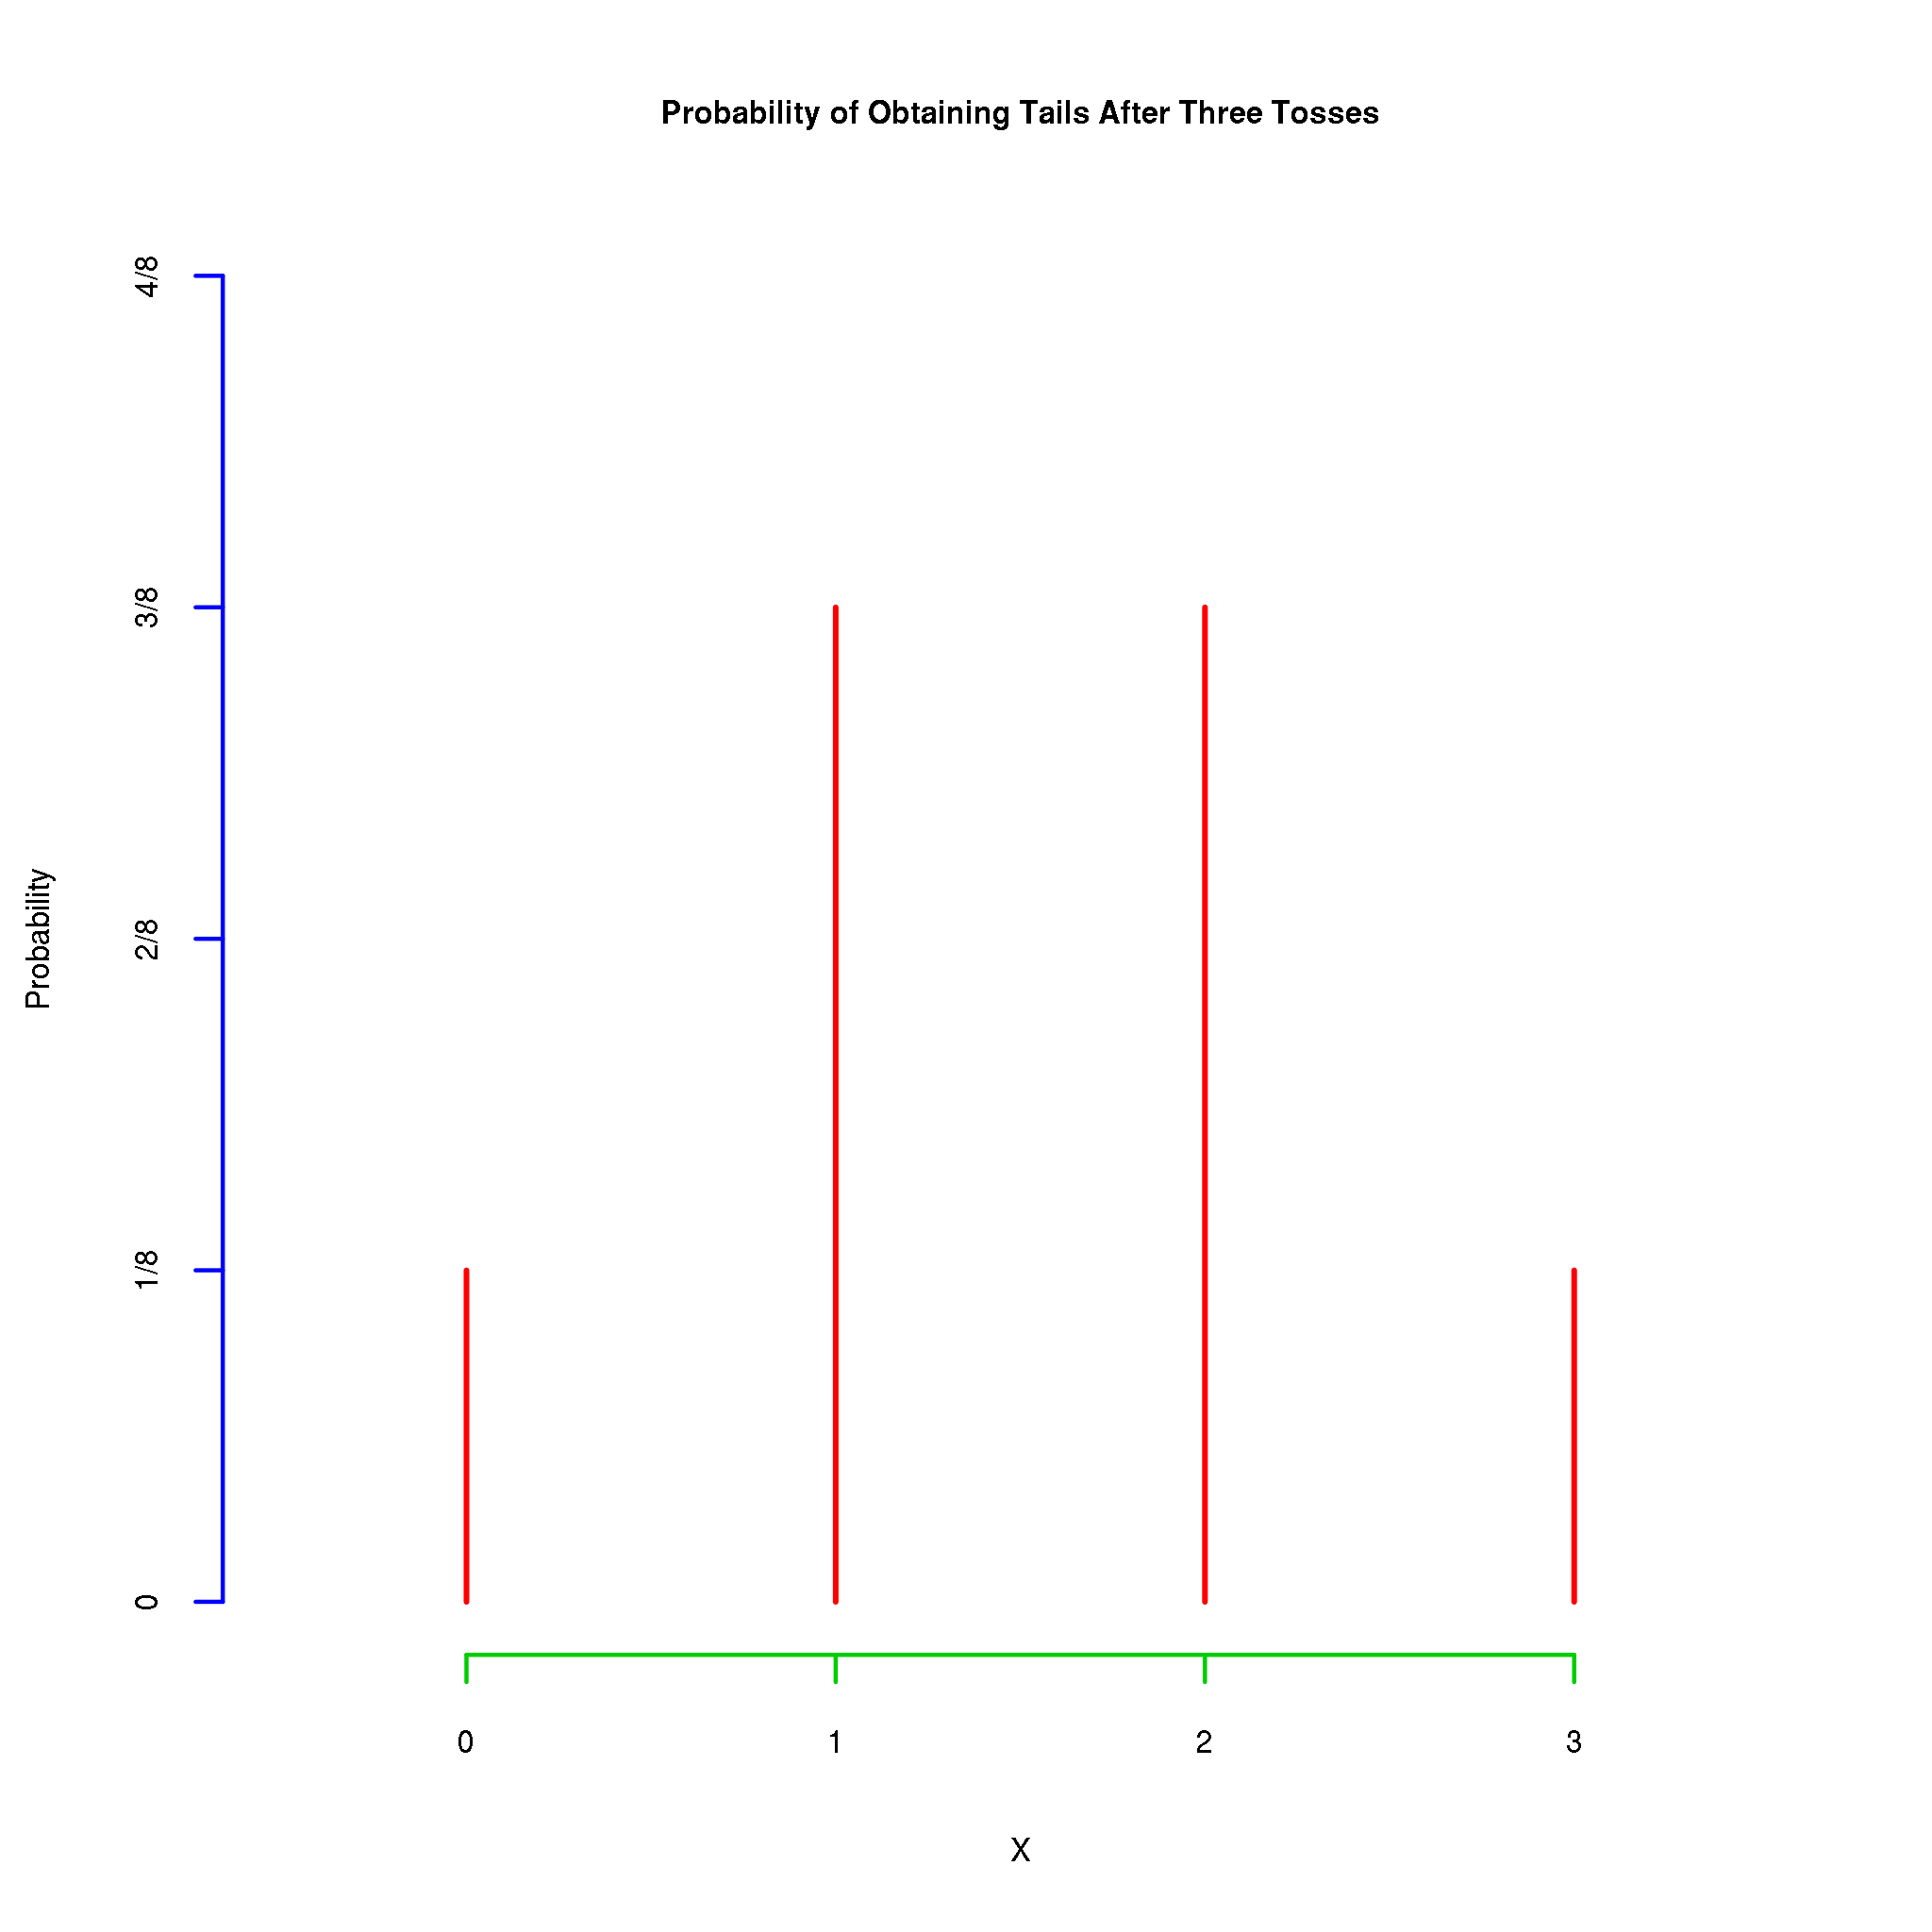
\includegraphics[width=6cm]{img/probDist3Tosses}

  \end{columns}
  
  
\end{frame}


\begin{frame}{Discrete Random Variables}

  \begin{columns}
    \column{.50\textwidth}

    The probability mass function (PMF):
    \begin{eqnarray*}
      \begin{array}{l|l}
        \mathrm{X} & p \\ \hline
        x_1 & p_1 \\
        x_2 & p_2 \\
        x_3 & p_3 \\
        \vdots & \vdots \\
        x_n & p_n
      \end{array}
    \end{eqnarray*}

    \column{.50\textwidth}
    Properties:
    \begin{eqnarray*}
      \begin{array}{rcccl}
        0 & \leq & p_i & \leq 1
      \end{array}
      \\
      p_1 + p_2 + p_3 + \cdots + p_n & = & 1.
    \end{eqnarray*}

  \end{columns}
  
\end{frame}


\begin{frame}{Discrete Random Variables}

  \begin{columns}
    \column{.15\textwidth}
    \begin{eqnarray*}
      \begin{array}{l|l}
        \mathrm{X} & p \\ \hline
        x_1 & p_1 \\
        x_2 & p_2 \\
        x_3 & p_3 \\
        \vdots & \vdots \\
        x_n & p_n
      \end{array}
    \end{eqnarray*}
    \vfill

    \column{.85\textwidth}
    \uncover<2->
    {
      \begin{definition}
        The \textbf{mean} of a random variable is
        \begin{eqnarray*}
          \mu_X & = & x_1 p_1 + x_2 p_2 + \cdots + x_n p_n.
        \end{eqnarray*}
      \end{definition}
    }

    \uncover<3->
    {
      \begin{definition}
        The \textbf{variation} of a random variable is
        \begin{eqnarray*}
          \sigma^2_X & = & (x_1-\mu_X)^2 p_1 + (x_2-\mu_X)^2 p_2 + \cdots + \\
                     &   & (x_{n-1}-\mu_X)^2 p_{n-1} + (x_n-\mu_X)^2 p_n.
        \end{eqnarray*}
      \end{definition}
    }

    \uncover<4->
    {
      \begin{definition}
        The \textbf{standard deviation} of a random variable is the
        square root of the variance.
      \end{definition}
    }

    
  \end{columns}
  
\end{frame}


\subsection{Examples}

\begin{frame}{Example}
  \begin{columns}
    \column{.15\textwidth}
    \begin{eqnarray*}
      \begin{array}{r|l}
        \mathrm{X} & p \\ \hline
        -2 & \frac{1}{6} \\ [5pt]
         0 & \frac{3}{6} \\ [5pt]
         2 & \frac{2}{6}
      \end{array}
    \end{eqnarray*}

    \column{.90\textwidth}
    \uncover<2->
    {
      \begin{eqnarray*}
        \mu_X & = & -2 \cdot \frac{1}{6} + 0 \cdot \frac{3}{6} + 2 \cdot \frac{2}{6}, \\
        & = & \frac{1}{3}.
      \end{eqnarray*}
    }

  \end{columns}

  \begin{eqnarray*}
    \uncover<3->{%
    \sigma^2_X & = & \lp -2-\frac{1}{3}\rp^2 \frac{1}{6} + 
                     \lp 0-\frac{1}{3}\rp^2 \frac{3}{6} + 
                     \lp 2-\frac{1}{3}\rp^2 \frac{2}{6}, \\
              & = & \frac{17}{9}, \\
    }
    \uncover<4->{%
    \sigma_X  & = & \sqrt{\frac{17}{9}}.
    }
  \end{eqnarray*}
  \vfill
    

\end{frame}



\begin{frame}{Clicker Quiz}

  What is the mean for the following probability distribution?
    \begin{eqnarray*}
      \begin{array}{r|l}
        \mathrm{X} & p \\ \hline
         0 & \frac{1}{8} \\ [5pt]
         1 & \frac{2}{8} \\ [5pt]
         2 & \frac{4}{8} \\ [5pt]
         3 & \frac{1}{8}
      \end{array}
    \end{eqnarray*}

    \vfill

  \begin{tabular}{l@{\hspace{3em}}l@{\hspace{3em}}l}
    A: 6/8  & B: 6/4 & C: 13/8
  \end{tabular}

  \vfill
  \vfill
  \vfill

\end{frame}

\begin{frame}{Example}
  \begin{columns}
    \column{.15\textwidth}
    \begin{eqnarray*}
      \begin{array}{r|l}
        \mathrm{X} & p \\ \hline
         0 & \frac{1}{8} \\ [5pt]
         1 & \frac{1}{8} \\ [5pt]
         2 & \frac{4}{8} \\ [5pt]
         3 & \frac{2}{8}
      \end{array}
    \end{eqnarray*}

    \column{.90\textwidth}
    \uncover<2->
    {
      \begin{eqnarray*}
        \mu_X & = & 0 \cdot \frac{1}{8} + 1 \cdot \frac{1}{8} + 2 \cdot \frac{4}{8} + 3 \frac{2}{8}, \\
        & = & \frac{15}{8}.
      \end{eqnarray*}
    }

  \end{columns}

  \begin{eqnarray*}
    \uncover<3->{%
    \sigma^2_X & = &  \lp 0-\frac{15}{8}\rp^2 \frac{1}{8} +  
                      \lp 1-\frac{15}{8}\rp^2 \frac{1}{8} + \\
               &    & \lp 2-\frac{15}{8}\rp^2 \frac{4}{8} + 
                      \lp 3-\frac{15}{8}\rp^2 \frac{2}{8}, \\
               & = & \frac{55}{64}. \\
     }
    \uncover<4->{%
        \sigma_X & = & \sqrt{\frac{55}{64}}.
    }
  \end{eqnarray*}
  \vfill

    

\end{frame}



% LocalWords:  Clarkson pausesection hideallsubsections
